\section{Motivation}
\label{sec:motivation}

%As mentioned in the introduction, besides the fact that performance test cases often involves larger inputs and thus consumes more resources and take more time, the performance variance among different executions of a same test case provides us an even stronger motivation for test prioritization in performance regression testing. 

%Theoretically, for each test case that does not involve random process (e.g., generating random numbers, randomly selecting next method invocations), all of its executions should go over exactly the same instruction sequence, and thus take exactly the same time. 

\begin{figure}
	\centering
	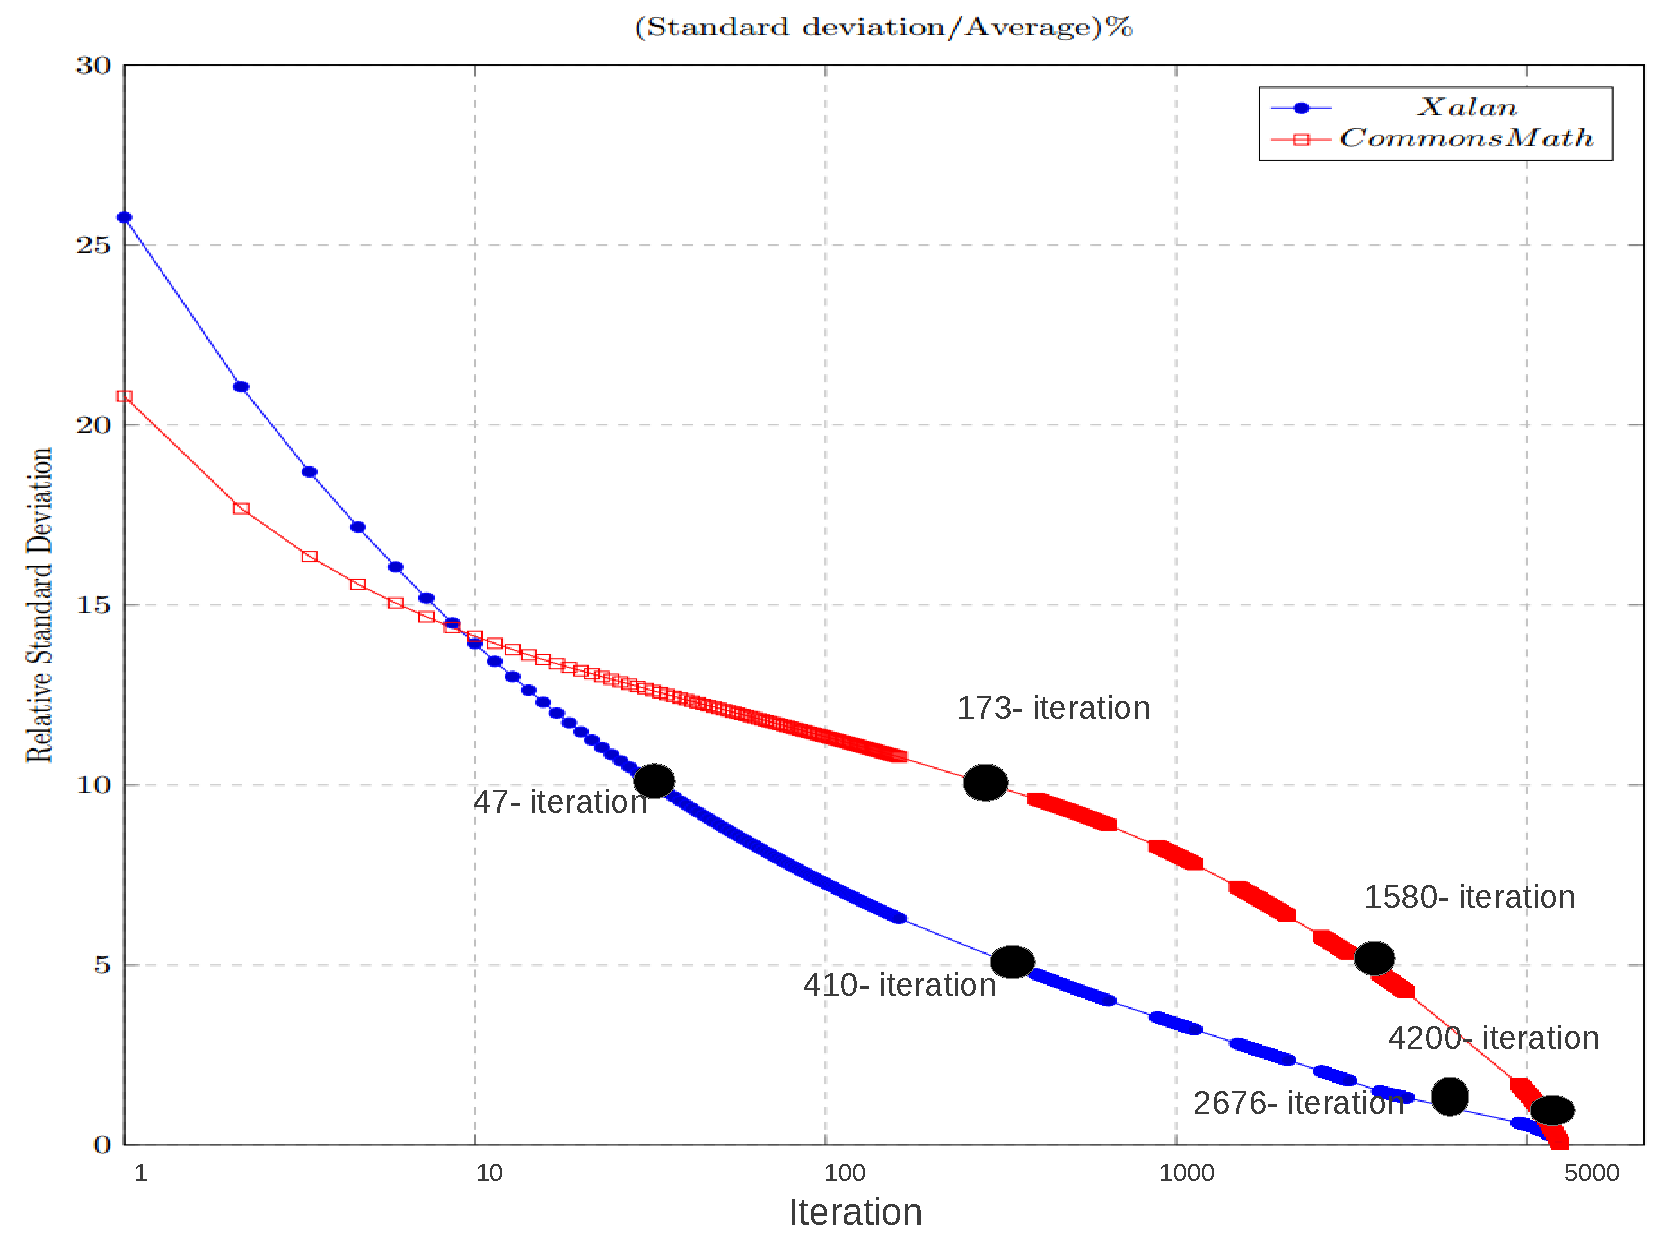
\includegraphics[width=0.45\textwidth]{performance/images/standard-deviation.pdf}
	\caption{Relative Standard Deviation vs. Sample Size}	
	\label{fig:motiv-math}	
	
\end{figure}

In this section, we provide preliminary study results to motivate prioritization of performance regression tests, due to high cost of executing the same test case for many times for performance regression testing. In particular, modern mechanisms in hardware and software often bring in random factors impacting performance. Some well-known examples are the randomness in scheduling cores and buses in multi-core systems~\cite{MultiCoreRandom}, in caching policies~\cite{CacheRandom}, and in the garbage-collection process~\cite{GBRandom}, etc. These factors interact with each other and amplify their effect so that the execution time of a test case may vary substantially from time to time. 

To neutralize such randomness, researchers or developers execute a test case multiple times and calculate the average performance~\cite{LiuCGO}. To better understand this requirement, we perform a motivating study (with more details on the project website~\cite{perfranker}) on the two open source projects used in evaluating our approach. In particular, we execute the test cases for 5,000 times, and randomly select samples with different sizes to calculate their standard deviation. In Figure~\ref{fig:motiv-math}, we show how the execution time's relative standard deviation (y axis) changes as the execution times (x axis) increase from 1 to 5,000. The figure shows that the average relative standard deviation with sample size 1 is over 20\% in both projects. In other words, if only one execution is used, the recorded execution time is expected to have more than 20\% difference from the average execution time in the 5,000 executions. Note that 20\% is a very large variance because 10\% performance enhancement is typically considered significant, and techniques incurring over 10\% overhead are often considered too slow for deployment purposes~\cite{DoubleTake}. The figure also shows that 173 and 47 executions are required to achieve relative standard deviation less than 10\% for Apache Commons Math and Xalan, respectively. Executing the whole test suite for many times can be prohibitively expensive, calling for prioritization of performance regression tests, as targeted by our approach. 


%The number of executions to acquire precise performance measurement may vary from scenario to scenario, and there is not a comprehensive study for it. In this paper, to understand how many executions are required to achieve precise result for our evaluation settings (i.e., performance testing of Java Projects on a state-of-the-art multi-core server), we performed a motivation study on the two test suite of our evaluation subjects: Apache Commons Maths and Xalan. 

%\textbf{Study Design.} For each project, we execute the test suite for 5,000 times on a quiet\footnote{``Quiet'' means that no other user process is running on the server.} DELL X630 server with 32 cores and 256GB memory. From the executions, for each test case, we recorded its execution time as a sequence with 5,000 data points\footnote{To avoid potential noises such as test-case loading or IO blocking, we removed the outliers that are beyond 2 times of standard deviation, which is a standard data purification process~\cite{}, and removed 0.9\% data points on average.}. In our study, we define ~\textit{Sample Size} as the number of iterations a test case is executed, and ~\textit{Sample Performance} as the average execution time calculated from the executions. For a small sample size (e.g., 1), the sample performance from different samples tends to have larger standard deviation, and when the sample size gets larger, the standard deviation among samples tends to get smaller, and our goal is to find the sample size that can lead to small enough standard deviation. 
%
%For each sample size $i$, we use all the sub-sequences with length $i$ of the original data-point sequence whose length is $N$\footnote{The value of $N$ is slightly smaller than 5,000 due to data purification.}
%
%Specifically, if the $k^{th}$ data point in the original data-point sequence is denoted as $ex(k)$, the first sample, the $k^{th}$ sample, and the last sample in the set will be:
%
%\begin{multline}
%sample(i, 1) = \{ex(1), ex(2), ...., ex(i)\}\\
%sample(i, k) = \{ex(k), ex(k+1$ $mod$ $N), ...., ex((k+i)$ $mod$ $N)\}\\
%sample(i, N) = \{ex(N), ex(1), ...., ex(i-1)\}\\
%\end{multline}
%
%Therefore, our sample set for sample size $i$ can be viewed as executing the test case for $i$ times from any start point in the original execution sequence. Based on these sample sets, if we denote the sample performance of $sample(i, k)$ as $perf(i, k)$, the relative standard deviation for sample size $i$ can be calculated as follows. 
%
%\begin{equation}
%Var(i) = \frac{Std(\cup{k=1}{N}{\{perf(i, k)\}\}})}{\Sigma{k=1}{N}{ex(k)}/N}
%\end{equation}
%
%In the formula, to normalize the standard deviation for different test cases and projects, we divide it with the average execution time of the test case for all $N$ executions. Therefore, we actually use the average execution time of the 5,000 executions to approximate the ideally precise execution time. It should be noted that, 5,000 is much larger than 10 to 100 which are common used in performance related research efforts in literature~\cite{}~\cite{}, so we believe that the approximation should be reasonably accurate.  For the sample sizes from 1 to 5000, we draw the trends of relative standard deviation (average for all test cases)
%\textbf{Study Results.} 


% 1,580 and 406 executions are required to achieve relative standard deviation less than 5\%. 



%in which horizontal axes represent sample sizes in log scale and vertical axes represent the relative standard deviation. 


%It should be noted that, our study has some limitations such as the purification of execution-time outliers which may exist in the real world testing, and the fact that sample sets are not independent with each other because there are overlaps between neighboring sample sets (e.g., $sample(i, 1)$ and $sample(i, 2))$. However, these two limitations will both reduce the observed relative standard deviation, indicating that we actually provided a lower bound of relative standard deviation over sample sizes. Therefore, as a motivation study, it show that we do need several hundred executions to confirm a performance regression around 10\%. Based on this fact, the prioritization of test cases is very helpful, because we can focus the highly prioritized test cases, and execute them for more times to better confirm perform regressions. 





%We can see that at first iteration average deviation from ideal is 20.79\% and reduced to 5\% with 1580 iteration. Finally the overall variance decreased to 1\% with iteration 4200. Furthermore, deviation decreases sharply from 20\% to 10\% with 173 times of execution whereas reduction from 10\% to 5\% take 1407 iteration. So we can say that large number of iteration of execution of test case are needed to get a stable execution time of a performance test case. A small extent of performance degradation may result in severe consequence motivate us that running performance test needs more time and resources. It is hard for a developer to understand performance impact with few runs.\\


%In the evaluation of techniques for compilers and systems, to reduce some randomness, researchers sometimes choose to turn off some features, such as doing garbage collection at fixed time point. However, 

%{\fontsize{7}{7}
%\begin{multline}
%\begin{gathered}
%Average = Avg(1,2,3,...,5000)\\
%Var(i) = \frac{ Std( Avg(1,2,...,i),...,Avg(5000,1,...,i-1))}{Average}\\
%Iteration(i) = \frac{ \sum \limits_{k=1}^{alltest} Var(i)}{alltest}
%\label{eq:eq-motivation}
%\end{gathered}
%\end{multline}
%}





%We run real test cases and captured average execution time of two popular open source project apache common math and xalan. \textbf{Common math}:  We chose 2703 test cases which are affected by code changes from a collection 3900 test cases and each of test cases  exercise 5000 time and record their execution time. In the formula ~\ref{eq:eq-motivation} function Avg and Std corresponding to average and standard deviation. For iteration-1, it becomes {\fontsize{7}{7}\[ Var(1) = \frac{Std(1,2,3,...,5000)}{Average}\]} which is fraction of standard derivation of 5000 data and average of 5000 data. The value of Var(1) represents how far the deviation is from the ideal case with a single iteration.For iteration-2, it becomes {\fontsize{7}{7} \[Var(2) = \frac{ Std( Avg(1,2), Avg(2,3),...,Avg(5000,1))}{Average}\]} where each data of standard deviation is average of 2 data which means that 2-iteration on the average how much deviate from ideal case. For iteration-5000, it becomes {\fontsize{7}{7}\[Var(5000) = \frac{ Std(Avg(1,2,...,5000),...,Avg(5000,1,...,4999))}{Average}\]} where each data of standard deviation is average of 5000 data which means Var(5000) value equals to zero that we considered as ideal or base case. According to the formula~\ref{eq:eq-motivation}, we generate a graph in the figure ~\ref{fig:common-math-motiv} 
